\documentclass{beamer}
\mode<presentation>
\usepackage{amsmath}
\usepackage{amssymb}
\usepackage{bm}
%\usepackage{advdate}
\usepackage{adjustbox}
\usepackage{subcaption}
%\usepackage{enumitem}
\usepackage{enumerate}
\usepackage{multicol}
\usepackage{mathtools}
\usepackage{listings}
\usepackage{url}
\def\UrlBreaks{\do\/\do-}
\usetheme{Boadilla}
\usecolortheme{lily}
\setbeamertemplate{footline}
{
  \leavevmode%
  \hbox{%
  \begin{beamercolorbox}[wd=\paperwidth,ht=2.25ex,dp=1ex,right]{author in head/foot}%
    \insertframenumber{} / \inserttotalframenumber\hspace*{2ex} 
  \end{beamercolorbox}}%
  \vskip0pt%
}
\setbeamertemplate{navigation symbols}{}

\providecommand{\nCr}[2]{\,^{#1}C_{#2}} % nCr
\providecommand{\nPr}[2]{\,^{#1}P_{#2}} % nPr
\providecommand{\mbf}{\mathbf}
\providecommand{\pr}[1]{\ensuremath{\Pr\left(#1\right)}}
\providecommand{\qfunc}[1]{\ensuremath{Q\left(#1\right)}}
\providecommand{\sbrak}[1]{\ensuremath{{}\left[#1\right]}}
\providecommand{\lsbrak}[1]{\ensuremath{{}\left[#1\right.}}
\providecommand{\rsbrak}[1]{\ensuremath{{}\left.#1\right]}}
\providecommand{\brak}[1]{\ensuremath{\left(#1\right)}}
\providecommand{\lbrak}[1]{\ensuremath{\left(#1\right.}}
\providecommand{\rbrak}[1]{\ensuremath{\left.#1\right)}}
\providecommand{\cbrak}[1]{\ensuremath{\left\{#1\right\}}}
\providecommand{\lcbrak}[1]{\ensuremath{\left\{#1\right.}}
\providecommand{\rcbrak}[1]{\ensuremath{\left.#1\right\}}}
\providecommand{\rank}{\text{rank}}
\theoremstyle{remark}
\newtheorem{rem}{Remark}
\newcommand{\sgn}{\mathop{\mathrm{sgn}}}
\providecommand{\abs}[1]{\left\vert#1\right\vert}
\providecommand{\res}[1]{\Res\displaylimits_{#1}} 
\providecommand{\norm}[1]{\lVert#1\rVert}
\providecommand{\mtx}[1]{\mathbf{#1}}
\providecommand{\mean}[1]{E\left[ #1 \right]}
\providecommand{\fourier}{\overset{\mathcal{F}}{ \rightleftharpoons}}
%\providecommand{\hilbert}{\overset{\mathcal{H}}{ \rightleftharpoons}}
\providecommand{\system}{\overset{\mathcal{H}}{ \longleftrightarrow}}
	%\newcommand{\solution}[2]{\vec{Solution:}{#1}}
%\newcommand{\solution}{\noindent \vec{Solution: }}
\providecommand{\dec}[2]{\ensuremath{\overset{#1}{\underset{#2}{\gtrless}}}}
\newcommand{\myvec}[1]{\ensuremath{\begin{pmatrix}#1\end{pmatrix}}}
\newenvironment{amatrix}[1]{%
  \left(\begin{array}{@{}*{#1}{c}|c@{}}
}{%
  \end{array}\right)
}
\let\vec\mathbf

\lstset{
%language=C,
frame=single, 
breaklines=true,
columns=fullflexible
}

%\numberwithin{equation}{section}

\title{Matgeo-q.1.4.14}
\author{AI25BTECH11039-Harichandana Varanasi}

\date{\today} 
\begin{document}

\begin{frame}
\titlepage
\end{frame}

\section*{Outline}


\begin{frame}
\frametitle{Question}
\item Points $A(-6,10)$, $B(-4,6)$ and $C(3,-8)$ are collinear such that 
\[
AB = \frac{2}{9}AC.
\]

\end{frame}
%
% --- FRAME 1 ---------------------------------------------------
\begin{frame}[t]{Solution}
\small
\textbf{Given:}\;
$\vec{A}=\myvec{-6\\10},\;
 \vec{B}=\myvec{-4\\6},\;
 \vec{C}=\myvec{3\\-8}.$

\medskip
\textbf{Assume:}\; $\vec{B}$ divides $\vec{A}\vec{C}$ in the ratio $k:1$.
\begin{align*}
\vec{B}&=\frac{k\vec{C}+\vec{A}}{k+1}
\end{align*}

\textbf{Compute }$k$:
\begin{align*}
k(\vec{B}-\vec{C})&=\vec{A}-\vec{B}\\[-2pt]
\Rightarrow\quad
k&=\frac{(\vec{A}-\vec{B})^\top(\vec{B}-\vec{C})}{\|\vec{B}-\vec{C}\|^2}
\end{align*}

\begin{align*}
\vec{A}-\vec{B}&=\myvec{-6\\10}-\myvec{-4\\6}=\myvec{-2\\4},\\[-2pt]
\vec{B}-\vec{C}&=\myvec{-4\\6}-\myvec{3\\-8}=\myvec{-7\\14},\\[-2pt]
\|\vec{B}-\vec{C}\|^2&=(-7)^2+14^2=245.
\end{align*}
\end{frame}

% --- FRAME 2 ---------------------------------------------------
\begin{frame}[t]{Solution}
\small
\textbf{Finish }$k$:
\begin{align*}
k&=\frac{\myvec{-2\\4}^{\!\top}\myvec{-7\\14}}{245}
=\frac{(-2)(-7)+(4)(14)}{245}
=\frac{70}{245}
=\boxed{\tfrac{2}{7}}
\end{align*}

\textbf{Ratios:}
\begin{align*}
AB:BC=\boxed{2:7},\qquad
\frac{AB}{AC}=\frac{2}{2+7}=\boxed{\tfrac{2}{9}}.
\end{align*}

\textbf{Check:}
\begin{align*}
\vec{B}
&=\frac{7\vec{A}+2\vec{C}}{9}
=\frac{7\myvec{-6\\10}+2\myvec{3\\-8}}{9}\\
&=\frac{\myvec{-42\\70}+\myvec{6\\-16}}{9}
=\frac{\myvec{-36\\54}}{9}
=\myvec{-4\\6}.
\end{align*}
\end{frame}
\begin{frame}{Graphical Representation}
   \begin{figure}[h!]
\centering
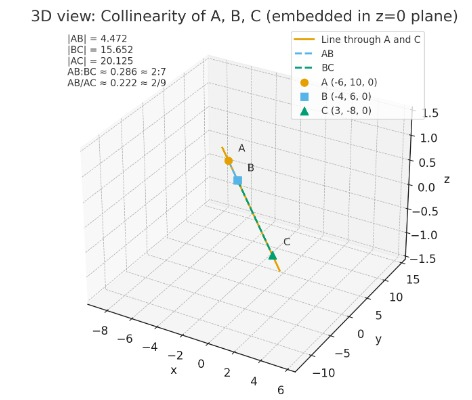
\includegraphics[width=0.7\linewidth]{figs/matgeo-1.4.14.jpeg}
\caption{3D view (embedded in $z=0$ plane) confirming collinearity}
\end{figure} 
\end{frame}

\end{document}
